\chapter*{Instructions to Authors}
\label{authorguide}

\subsection{Audience}
Refer to the \emph{Author-Audience Matrix}.
\begin{figure}[h]
\centering
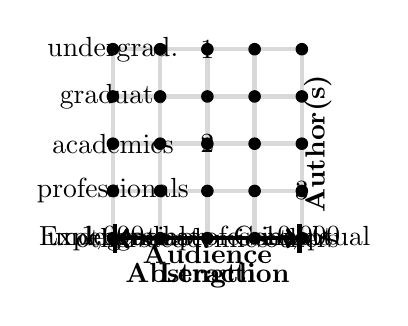
\begin{tikzpicture}[pubaxis/.style={font=\bfseries\scshape}]
  \draw[draw=gray!30,ultra thick,step=6mm] (0,0) grid (24mm,24mm);
  \foreach \x in {0,6,...,24}
    \foreach \y in {0,6,...,24}
      \fill (\x mm,\y mm) circle (0.8mm);
  \path;
  { [every node/.style={anchor=north west,scale=0.8}]
    \node at (12mm,24mm) {1};
    \node at (12mm,12mm) {2};
    \node at (24mm,6mm) {3};
  }
  { [every node/.style={inner sep=3mm}]
    { [shift={(0,24mm)},every node/.style={anchor=base west,rotate=60}]
      \node at (0,0) {undergrad.};
      \node at (6mm,0) {graduate};
      \node at (12mm,0) {academics};
      \node at (18mm,0) {professionals};
      \node at (24mm,0) {others};
    }
    { [every node/.style={anchor=mid east}]
      \node at (0,24mm) {undergrad.};
      \node at (0,18mm) {graduate};
      \node at (0,12mm) {academics};
      \node at (0,6mm) {professionals};
      \node at (0,0) {others};
    }
    { [every node/.style={anchor=north}]
      \node [pubaxis,rotate=90] at (26mm,12mm) {Author(s)};
      \node [pubaxis] at (12mm,-2mm) {Audience};
    }
  }
  { [shift={(42mm,3mm)}]
    \draw [|<->|,ultra thick] (0,0) -- (24mm,0);
    \node [pubaxis,anchor=north] at (12mm,-2mm) {Length};
    { [every node/.style={anchor=south,inner sep=3mm,scale=0.8}]
      \node at (0,0) {1,000};
      \node at (24mm,0) {10,000};
    }
  }
  { [shift={(42mm,18mm)}]
    \draw [|<->|,ultra thick] (0,0) -- (24mm,0);
    \node [pubaxis,anchor=north] at (12mm,-2mm) {Abstraction};
    { [every node/.style={anchor=south,inner sep=3mm,scale=0.8}]
      \node at (0,0) {Experiential};
      \node at (24mm,0) {Conceptual};
    }
  }
\end{tikzpicture}
\caption{\textsc{Author-Audience Matrix.} (1) includes student coursework, (2) includes most technical journals, and (3) could be engineering consultants reporting to a client firm.}
\end{figure}
Identify which row (or rows, for mixed groups of co-authors) you inhabit, and then make a choice of which audience your article will address.
We encourage you to share lessons and insights which are broadly reusable (i.e. cover two or more points), but it is critical that \emph{ELR} editors are able to discern your choice.
Either note your audience choice when submitting, or make some explicit reference to it in your text.

\subsection{Format, length \& language}
Choose a target length in increments of 500 words.
One thousand words is a rough (but not absolute) minimum.
\emph{ELR} prefers long-format writing; give your whole thoughts, not just sketches of them.

\emph{ELR} accepts submissions in Canadian English and French.

\subsection{Reviews \& revisions}
Articles are subject to double-blind reviews; the author(s) are anonymous to the reviewers and vice versa.
Where possible the reviewers will be from the audience chosen by the author(s).

Reviewers have the option to recommend an article be resubmitted for review, in which case a second review is undertaken after revisions have taken place.
Otherwise an \emph{ELR} Section Editor will coordinate revisions with author(s) and recommend acceptance to the Editorial Board once (s)he judges the reviewers' concerns are satisfied.

The Editorial Board may reject any article, postpone it for publication in a later issue, or request a resubmission, on the basis of reviews or any other cause.

\subsection{License \& republication}
\emph{ELR} prefers submissions which have not been published in the same form elsewhere.
However, the compilation or abridgement of existing works, where such compilation or abridgement makes the resulting text valuable to the readership of \emph{ELR}, is acceptable.

\emph{ELR} does \emph{not} ask or require that authors cede ownership or copyright of their work.
However, in the interest of preventing barriers to accessing the much-needed discussion on engineering leadership, \emph{ELR} requires authors to license their work under one of the Creative Commons licenses, all of which preserve the core right of readers to redistribute the work for non-commercial purposes without modification.

We suggest the most liberal (`Attribution') license, but authors may select another license at their discretion. Authors can learn more about the Creative Commons licenses at \url{http://creativecommons.org/choose/?jurisdiction=ca}

\subsection{Graphics}
Black-and-white and greyscale graphics are welcome accompaniment to articles, especially where they clearly illustrate the frameworks and conceptual relationships discussed therein.
The \emph{ELR} layout and graphic design staff can assist authors in converting sketches and colour graphics into suitable formats and resolutions for printing.

\subsection{Technical}
\emph{ELR} is published in \LaTeX; accordingly, submissions in \LaTeX~ format are preferred where possible.
However, \emph{ELR} can review and copyedit articles in most common document formats, including:
\begin{itemize}
  \item Open Document Format (ODF)
  \item Rich Text Format (RTF)
  \item Plain text, and
  \item Microsoft Word format.
\end{itemize}
The outcome of editorial decisions is not affected by the format of a submission.

Complete bibliographic information should accompany each article.
If possible, such information should be in BibTeX format.
Otherwise, authors should not exert themselves to follow any particular bibliographic format, but simply ensure the connection of particular citations to the cited items are clear.

All open and many common proprietary graphics formats are accepted.
